\section{Problem 2B: Stochastic SIR model}

\subsection{a)}

As seen in the plot in figure \ref{fig:SIR_stoch}, the $10$ different realisations of the stochastic SIR model , shown in dashed lines in graded colours, seem to lie close to the deterministic solution.

\begin{figure}[htb]
	\centering
	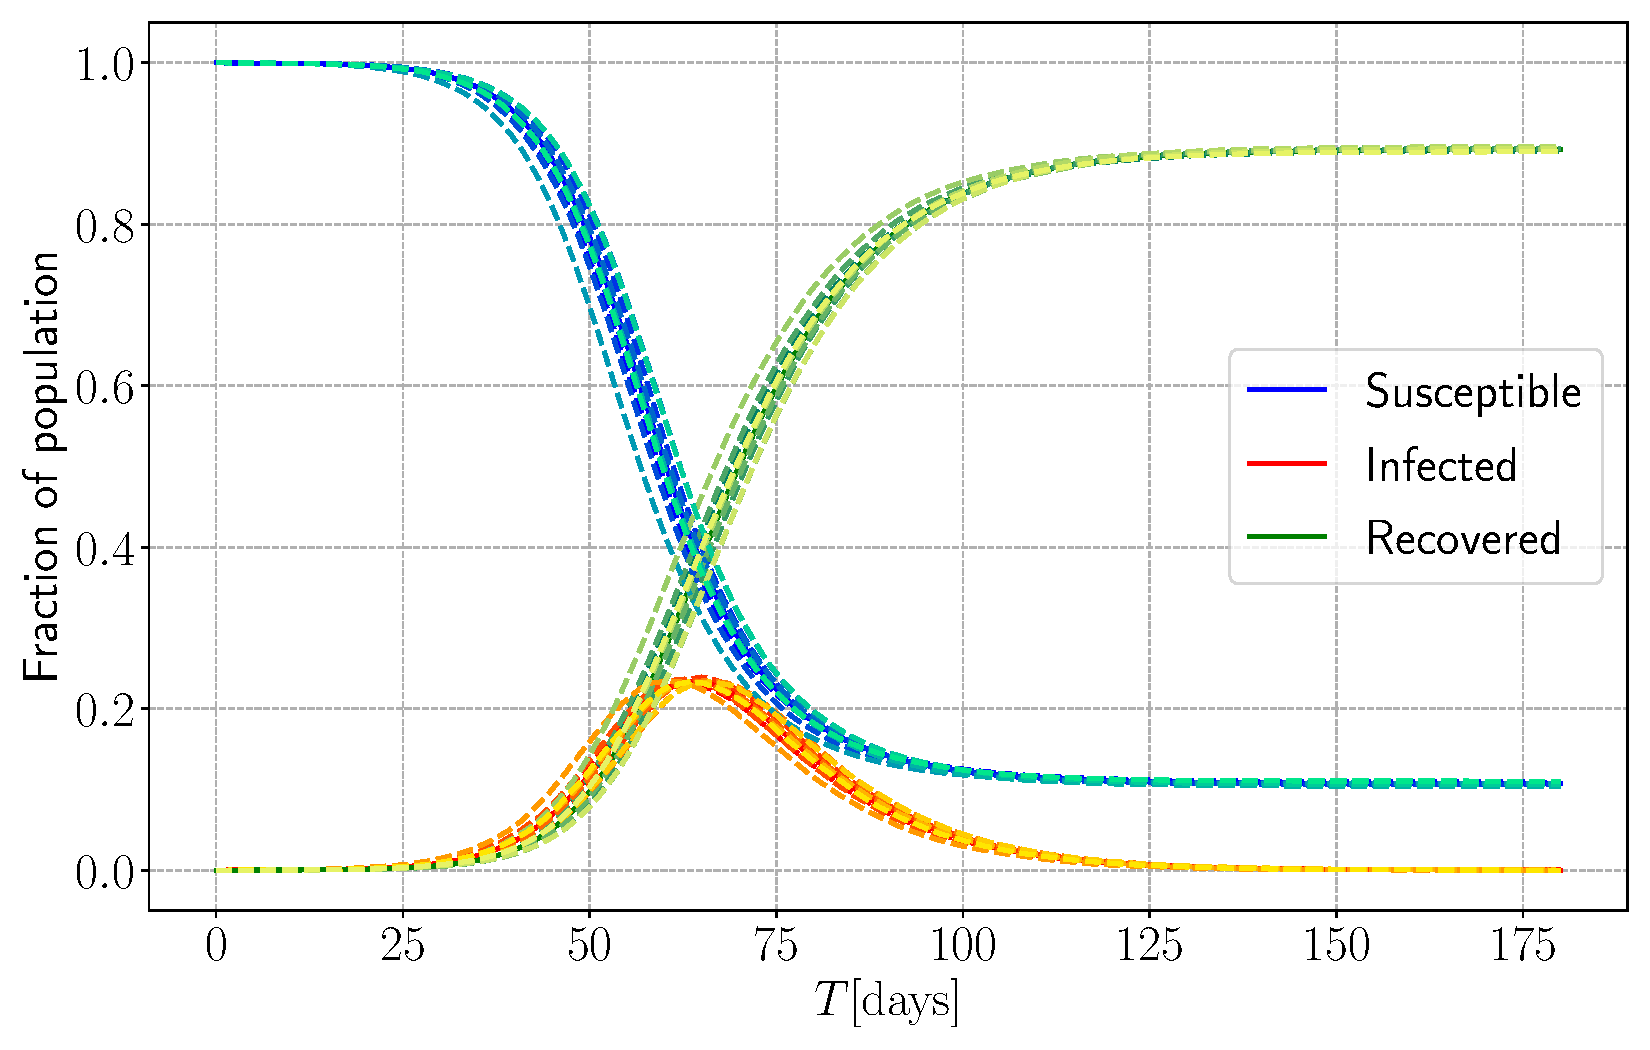
\includegraphics[width=0.8\columnwidth]{../fig/2Ba_SIR.pdf}
	\caption{Solution of stochastic SIR equations with $\beta = 0.25\, \mathrm{day}^{-1}$, $\tau = 10\, \mathrm{day}$.}
	\label{fig:SIR_stoch}
\end{figure}

To choose a suitable time-step for simulating this model, I run the simulation up to $t = 250$ days and find the deviation between the fraction of susceptible and the semi-analytic expression given in the problem sheet \cite{sheet}, and similarly for the fraction of recovered. I include the same run with the deterministic model to see how the deviations relate to each other. This is shown in figure \ref{fig:timesteps}. Clearly, using this comparison is \textit{not} a good way of determining the time step we want to use for the deterministic model, as the solution approaches the asymptotic values for all of the step lengths. However, we see from this plot that if we choose a step length $\lesssim 0.01$, the deviations of the stochastic solutions start to flatten out, and are roughly of the same order as those of the deterministic model. I therefore always use a time step smaller than $0.01$ for simulating the stochastic models. In particular, I use $\Delta t = 0.005$ in problem B,C,D and Ea. For Eb I use $\Delta t = 0.01$ because the runtime become uncomfortably large when using smaller time steps.

\begin{figure}[htb]
	\centering
	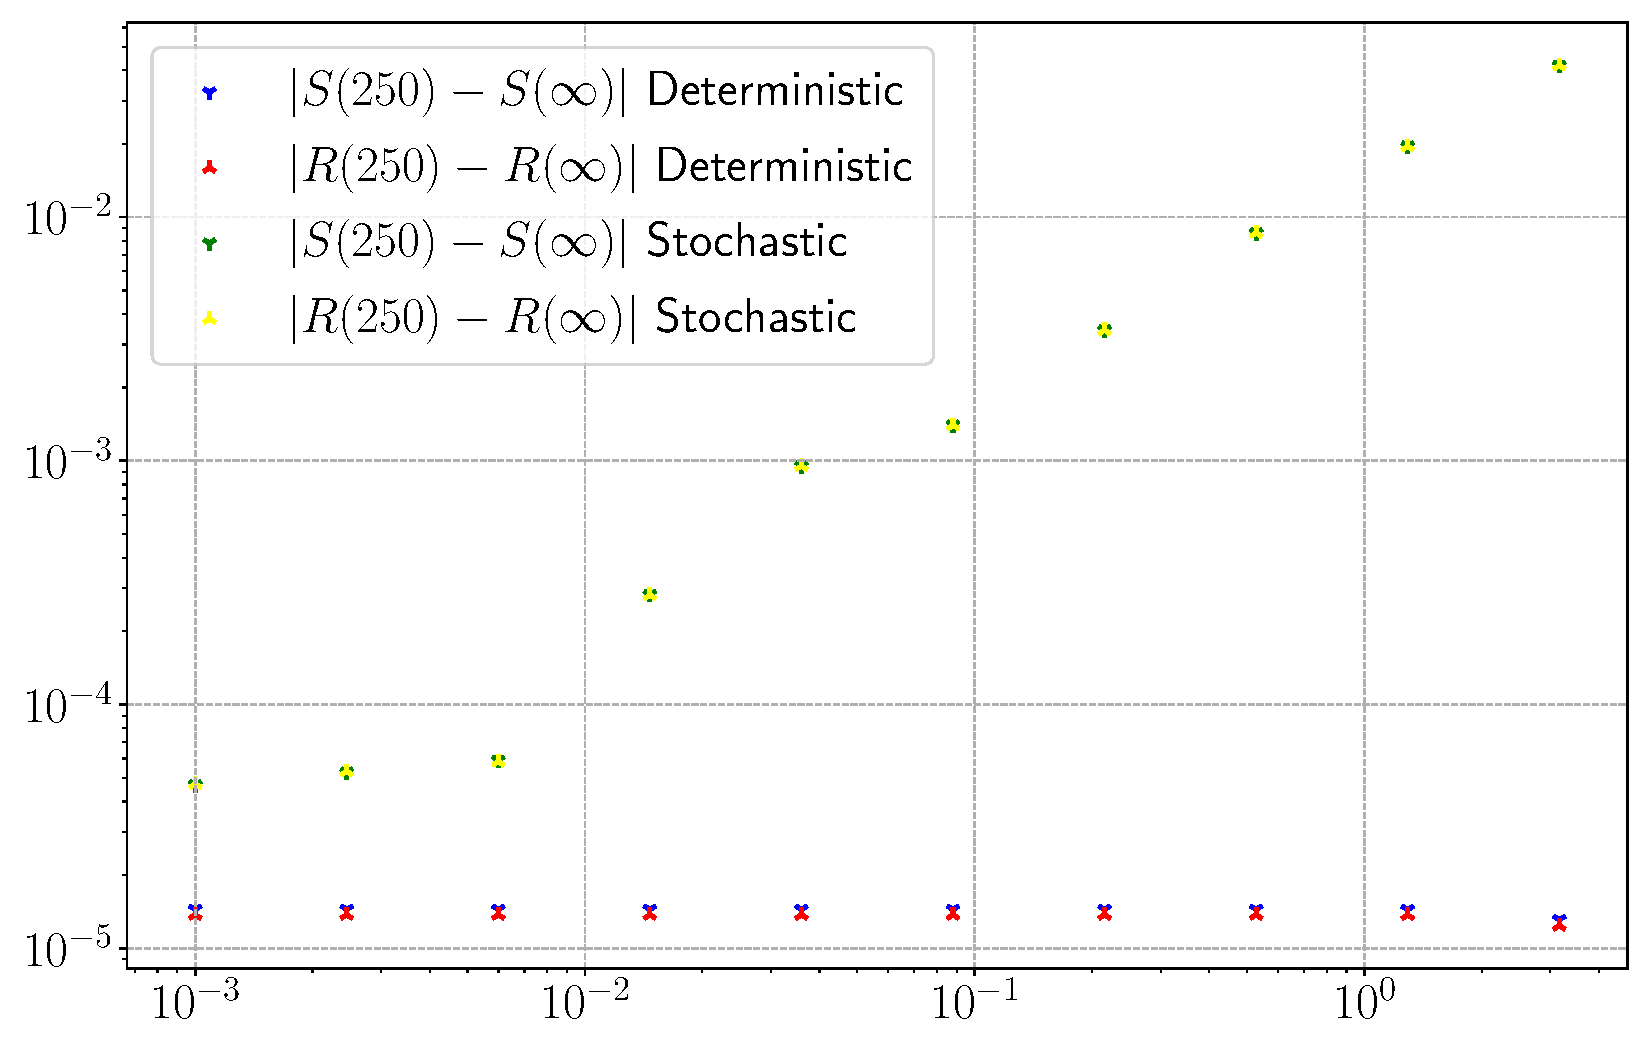
\includegraphics[width=0.8\columnwidth]{../fig/timestep.pdf}
	\caption{Deviations between the semi-analytical expressions for the asymptotic value.}
	\label{fig:timesteps}
\end{figure}

\subsection{b)}

As in the previous exercise, we plot the fraction of infected people together with the analytical model for the early stages. This is shown in figure \ref{fig:Infected_stoch}. Here we clearly see that all the realisations are approximately linear in the semi-log plot in the first $40$ days, or so, of the simulation as we observed in the previous exercise. 

\begin{figure}[htb]
	\centering
	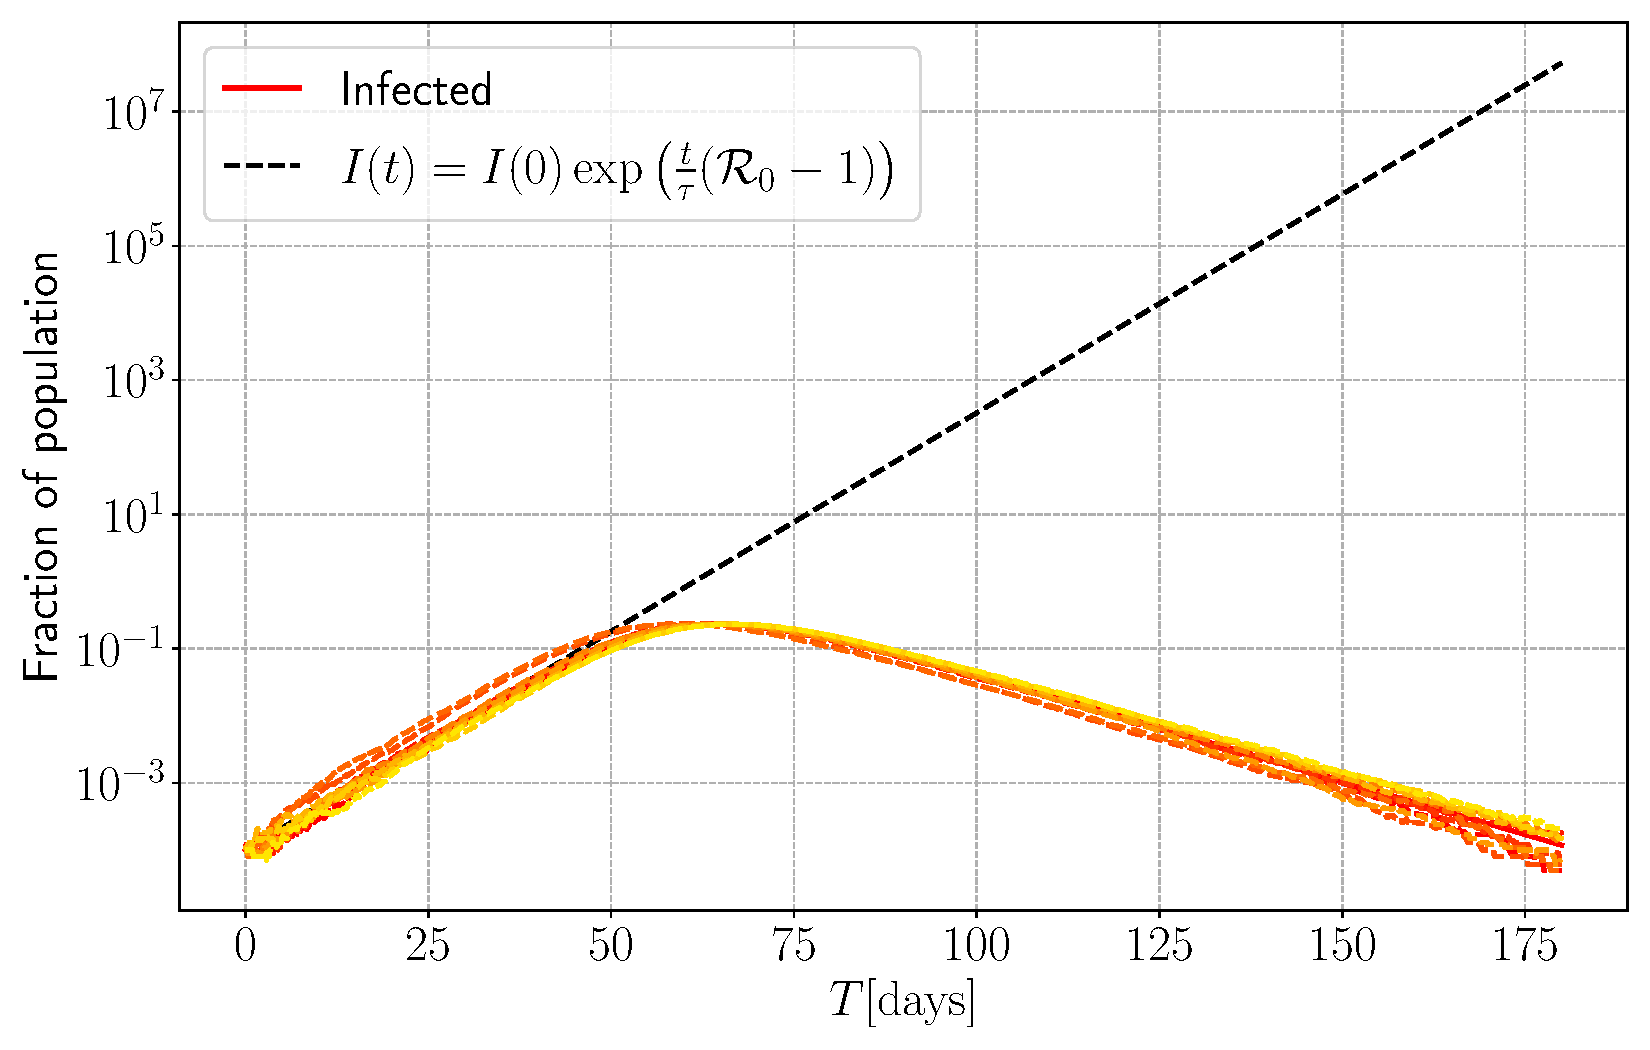
\includegraphics[width=0.8\columnwidth]{../fig/2Bb_I.pdf}
	\caption{Infected people compared with the analytical approximation at the early stages. Stochastic and deterministic model.}
	\label{fig:Infected_stoch}
\end{figure}

\subsection{c) Probability of an outbreak}

There will always be a certain probability for an outbreak disappearing by itself for the stochastic model. In the present subsection we estimate this probability for an initial number of infected people $=1,2,\dots,10$. This is done by the procedure described in algorithm \ref{alg:prob_I}.

\begin{algorithm}[htb]
	Choose the parameters of the model as those given in the exam sheet \cite{sheet}, but with $T = 30 \, \mathrm{days}$\footnote{As the typical infection time is $10$ days, I assume 50 days to be sufficient for detecting an outbreak in the stochastic model.}. \;
	Choose a batch-size $B$.\;
	\For{$I = 1,2,\dots, 10$}{
		Initialise an empty vector of length $B$: $\mathbf{X} = [0,\dots,0]$.\;
		\For{$n = 1,\dots, B$}
			{
			Run the simulation with initial number of infected people $= I$.\;
			Calculate the \texttt{slope} in the semi-log axes for $I(t)$.\;
			\eIf{$\texttt{slope} <= 0$}
			{$X_n = 0$}
			{$X_n = 1$}
		}
		Estimate the probability of an outbreak for $I$ initially infected by 
		$$
				p \coloneqq P(\mathrm{outbreak}|I) = \frac{1}{B} \sum_{n= 1}^{B} X_n. \;
		$$	
		Calculate the standard deviation of the estimate by 
		\begin{equation}\label{eq:std}
			\sqrt{\mathrm{Var}(\hat{p})} = \sqrt{\frac{p(1-p)}{B}}.
		\end{equation}
	}
	\caption{Calculating the probability of an outbreak as a function of the initial number of infected people, $I$. }
	\label{alg:prob_I}
\end{algorithm} 

In performing this procedure, I use a batch size of $500$ in each sweep. What we are estimating here is essentially a Bernoulli-distributed random variable, $X$: $X$ can take the realisations $1$ or $0$ with probabilities $p$ and $1-p$ respectively, and we assume them to be independent \cite[~p.26]{Wassermann}. Then, as the variance of such a distribution is $p(1-p)$, the variance of the estimator for the probability, namely $\hat{p}$\footnote{That is, the mean value of $X_n$.} is 
$$
	\mathrm{Var}(\hat{p}) =  \sum_{n= 1}^{B} \mathrm{Var}\left(\frac{X_n}{B}\right) = \frac{1}{B^2} \sum_{n= 1}^{B} \mathrm{Var}(X_n) = \frac{1}{B^2} \sum_{n= 1}^{B} p (1-p) = \frac{p(1-p)}{B},
$$
from which formula \eqref{eq:std} follows. 

The probability of an outbreak as a function of the initial number of infected people are shown in figure \ref{fig:prob_outbreak} together with the associated standard deviation. As seen from this plot, when there are more than $6$ people initially infected, the probability is approximately $1$ that an outbreak will happen. However, for e.g. $1$ initially infected person, the probability is less than $0.6$. This ultimately shows that the stochastic model has a more realistic feature to it than the deterministic one, in that these scenarios might occur.
% The probabilities are also shown in table \ref{tab: probabilities}

\begin{figure}[htb]
	\centering
	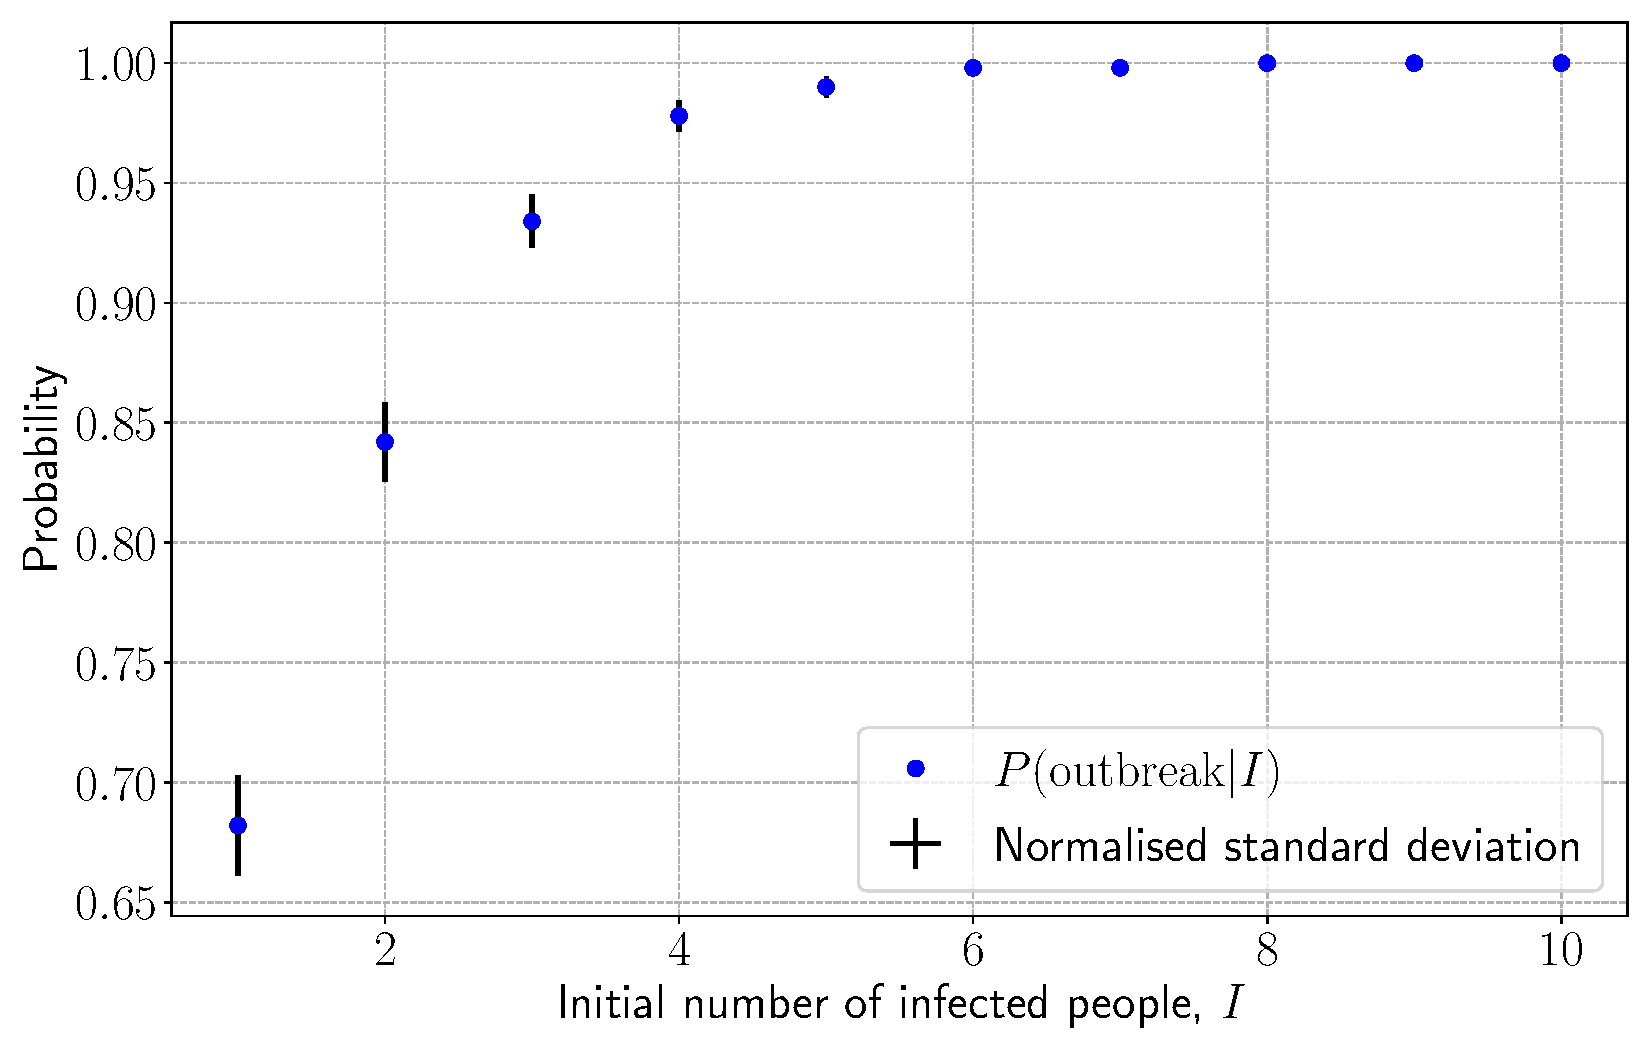
\includegraphics[width=0.8\columnwidth]{../fig/2Bc_prob.pdf}
	\caption{Probability of an outbreak as a function of initial number of infected people.}
	\label{fig:prob_outbreak}
\end{figure}

\clearpage